\documentclass{article}
\usepackage[utf8]{inputenc}
\usepackage{algorithmicx, algpseudocode, algorithm}
\usepackage{tikz}
\usepackage{amsmath}
\usepackage{amsthm}
\usepackage{multicol}
\usepackage{amssymb}
\usepackage[paper=a4paper, left=1.5cm, right=1.5cm, bottom=1.5cm, top=1.5cm]{geometry}
\usepackage{xcolor}

\title{}
\author{}
\date{}

\begin{document}

\section*{A tener en cuenta:}

\subsubsection*{Ecuación de calor:}

\[\frac{\partial^2 T(r,\theta)}{\partial r^2} + 
\frac{1}{r}\frac{\partial T(r,\theta)}{\partial r} + 
\frac{1}{r^2}\frac{\partial^2 T(r,\theta)}{\partial \theta^2} = 0\]

\

\noindent \small{(los puntos internos del horno cumplen con esta ecuación de calor)}

\subsubsection*{Discretización:}

\[\frac{t_{j-1,k} - 2t_{j,k} + t_{j+1,k}}{{(\Delta r)}^2} + 
\frac{1}{r_j}\frac{t_{j,k} - t_{j-1,k}}{\Delta r} + 
\frac{1}{r_{j}^{2}}\frac{t_{j,k-1} - 2t_{j,k} + t_{j,k+1}}{{(\Delta \theta)}^2} = 0\]

\subsubsection*{Función}

\begin{itemize}
    \item[-] $T(r,\theta)~:~\mathbb{R}^{2} \to \mathbb{R}$
    \item[-] $T(r_j, \theta_j) = t_{j,k}$
    \item[-] $T(r_i, \theta) = T(r_0, \theta) = T_i = 1500$
    \item[-] $T(r_m, \theta) = T(r_e, \theta) = T_{e}(\theta)$
\end{itemize}

\subsection*{Más datos:}

\subsubsection*{Discretización en ángulos}
\begin{itemize}
    \item[-] Una partición $0 = \theta_{0} < \theta_{1} < \cdots < \theta_{n} = 2\pi$ en $n$ ángulos discretos con
            $\theta_{k} - \theta_{k-1} = \Delta\theta$ para $k=1,\ldots,n$.
\end{itemize}

\subsubsection*{Discretización en radios}
\begin{itemize}
    \item[-] Una partición $r_i = r_0 < r_{1} < \cdots < r_{m} = r_e$ en $m+1$ radios discretos con
            $r_{j} - r_{j-1} = \Delta r$ para $j=1,\ldots,m$.
\end{itemize}

\subsubsection*{Representación}
Se pretende obtener una matriz $A \in \mathbb{R}^{n\times n}$ como matriz del sistema.

\subsubsection*{Entrada del problema}
El input será la tupla $(r_i, r_e, m+1, n,\text{valor de la isoterma buscada},T_i,T_e(\theta))$, donde cada elemento representa:
\begin{itemize}
    \item[-] $r_i$: valor del radio interno 
    \item[-] $r_e$: valor del radio externo
    \item[-] $m+1$: cantidad de radios
    \item[-] $n$: ángulos
    \item[-] $T_i$: valor de $T$ (temperatura) en $r_i$ en cualquier ángulo
    \item[-] $T_e(\theta)$: valor de $T$ (temperatura) en $r_e$ para cada ángulo $\theta$
\end{itemize}

\subsubsection*{Salida del problema}
\indent \indent Se busca $T(r,\theta)$ para todo punto de la pared del horno 
$(r_i \leq r \leq r_e~\text{y}~ \theta\in[0,2\pi])$, 
de forma que se puede encontrar donde está la isoterma buscada.


\newpage


\section*{Ejemplos}

\subsection*{Ejemplo trivial}

Tomo como input del problema la tupla:
\begin{itemize}
    \item[-] $(6, 10, 3, 2, 500, 1500, (200,200,200))$
\end{itemize}

\noindent es decir: 

\begin{itemize}
    \item[-] $r_i = 6 = r_0$ 
    \item[-] $r_e = 10 = r_2$
    \item[-] $m+1 = 3$
    \item[-] $n = 2$
    \item[-] Isoterma buscada = $500$ 
    \item[-] $T_i = 1500$
    \item[-] $T_e(\theta) = (200,200,200) \to \theta_0 = 200,~\theta_1 = 200, ~\theta_2 = \theta_n = 200$
\end{itemize}

\subsubsection*{Discretización}


\begin{center}
    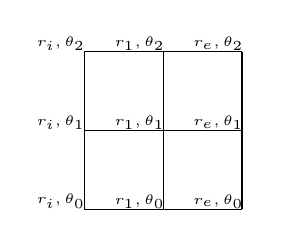
\begin{tikzpicture}
        \draw[black] (0,0) grid (2,2);
        \node at (-0.3,2.1) {\tiny{$r_i,\theta_2$}};
        \node at (-0.3,1.1) {\tiny{$r_i,\theta_1$}};
        \node at (-0.3,0.1) {\tiny{$r_i,\theta_0$}};

        \node at (0.7,2.1) {\tiny{$r_1,\theta_2$}};
        \node at (0.7,1.1) {\tiny{$r_1,\theta_1$}};
        \node at (0.7,0.1) {\tiny{$r_1,\theta_0$}};

        \node at (1.7,2.1) {\tiny{$r_e,\theta_2$}};
        \node at (1.7,1.1) {\tiny{$r_e,\theta_1$}};
        \node at (1.7,0.1) {\tiny{$r_e,\theta_0$}};
    \end{tikzpicture}
\end{center}    

\subsubsection*{Visto como matriz}

\begin{center}
    \begin{tabular}{ |c|c|c| }
        \hline
        $r_0,\theta_2$ & $r_1,\theta_2$ & $r_2,\theta_2$ \\
        \hline
        $r_0,\theta_1$ & $r_1,\theta_1$ & $r_2,\theta_1$ \\
        \hline
        $r_0,\theta_0$ & $r_1,\theta_0$ & $r_2,\theta_0$ \\
        \hline
    \end{tabular}
\end{center}

\subsubsection*{Datos e incognitas:}

\begin{multicols}{3}
    \begin{itemize}
        \item[] $T(r_0,\theta_2) = t_{02} = 1500$
        \item[] $T(r_0,\theta_1) = t_{01} = 1500$
        \item[] $T(r_0,\theta_0) = t_{00} = 1500$
    \end{itemize}

    \begin{itemize}
        \item[] $T(r_1,\theta_2) = t_{12} =~$?
        \item[] $T(r_1,\theta_1) = t_{11} =~$?
        \item[] $T(r_1,\theta_0) = t_{10} =~$?
    \end{itemize}

    \begin{itemize}
        \item[] $T(r_2,\theta_2) = t_{22} = 200$
        \item[] $T(r_2,\theta_1) = t_{21} = 200$
        \item[] $T(r_2,\theta_0) = t_{20} = 200$
    \end{itemize}
\end{multicols}

\subsubsection*{Resolución}

Para resolver el problema planteo la ecuación de calor para cada punto interno:

\

\begin{align*}
    \textcolor{magenta}{T(r_1,\theta_1)} = 
    \frac{t_{01} - 2t_{11} + t_{21}}{{(\Delta r)}^{2}} + 
    \frac{1}{r_1}\frac{t_{11} - t_{01}}{\Delta r} + 
    \frac{1}{r_{1}^{2}}\frac{t_{10} - 2t_{11} + t_{12}}{{(\Delta\theta)}^2} &= 0 \\
    %
    {(\Delta r)}^{-2}[t_{01} - 2t_{11} + t_{21}] + 
    {(r_1\Delta r)}^{-1}[t_{11} - t_{01}] + 
    {(r_{1}\Delta \theta)}^{-2}[t_{10} - 2t_{11} + t_{12}] &= 0 \\
    %
    {(\Delta r)}^{-2}t_{01} - {(\Delta r)}^{-2}2t_{11} + {(\Delta r)}^{-2}t_{21} + 
    {(r_1\Delta r)}^{-1}t_{11} - {(r_1\Delta r)}^{-1}t_{01} + 
    {(r_{1}\Delta \theta)}^{-2}t_{10} - {(r_{1}\Delta \theta)}^{-2}2t_{11} + {(r_{1}\Delta \theta)}^{-2}t_{12} &= 0 \\
    %
    {(\Delta r)}^{-2}t_{01} - {(r_1\Delta r)}^{-1}t_{01} + {(r_{1}\Delta \theta)}^{2}t_{10} 
    - {(\Delta r)}^{-2}2t_{11} + {(r_1\Delta r)}^{-1}t_{11} - {(r_{1}\Delta \theta)}^{-2}2t_{11} 
    + {(r_{1}\Delta \theta)}^{-2}t_{12} + {(\Delta r)}^{-2}t_{21} &= 0 \\
    %
    [{(\Delta r)}^{-2} - {(r_1\Delta r)}^{-1}]t_{01} + [{(r_{1}\Delta \theta)}^{-2}]t_{10} 
    + [{(r_1\Delta r)}^{-1} - 2{(\Delta r)}^{-2} - 2{(r_{1}\Delta \theta)}^{-2}]t_{11} 
    + [{(r_{1}\Delta \theta)}^{-2}]t_{12} + [{(\Delta r)}^{-2}]t_{21} &= 0 \\
\end{align*}

\noindent Cada punto interno tendrá la siguiente ecuación (teniendo en cuenta que varían los indices):

\begin{align*}
    \frac{-[{(\Delta r)}^{-2} - {(r_1\Delta r)}^{-1}]t_{01} - [{(r_{1}\Delta \theta)}^{-2}]t_{10} 
    - [{(r_{1}\Delta \theta)}^{-2}]t_{12} - [{(\Delta r)}^{-2}]t_{21}}
    {[{(r_1\Delta r)}^{-1} - 2{(\Delta r)}^{-2} - 2{(r_{1}\Delta \theta)}^{-2}]} - t_{11} &= 0 \\
    %
    \textcolor{magenta}{
    -\frac{[{(\Delta r)}^{-2} - {(r_1\Delta r)}^{-1}]}{[{(r_1\Delta r)}^{-1} - 2{(\Delta r)}^{-2} - 2{(r_{1}\Delta \theta)}^{-2}]}t_{01}}
    & \\
    \textcolor{magenta}{
    -\frac{[{(r_{1}\Delta \theta)}^{-2}]}{[{(r_1\Delta r)}^{-1} - 2{(\Delta r)}^{-2} - 2{(r_{1}\Delta \theta)}^{-2}]}(t_{10} + t_{12})
    -\frac{[{(\Delta r)}^{-2}]}{[{(r_1\Delta r)}^{-1} - 2{(\Delta r)}^{-2} - 2{(r_{1}\Delta \theta)}^{-2}]}t_{21} - t_{11}} &~\textcolor{magenta}{= 0}
\end{align*}

\newpage

\noindent Dado que el valor de los radios, angulos y diferenciales es conocido: 

\begin{itemize}
    \item[-] $r_1 = 8$
    \item[-] $\Delta r = 2$ 
    \item[-] $\Delta\theta = \pi$,
\end{itemize}

procedo a calcular los coeficientes de las incognitas:

\begin{align*}
    -\frac{[{(\Delta r)}^{-2} - {(r_1\Delta r)}^{-1}]}{[{(r_1\Delta r)}^{-1} - 2{(\Delta r)}^{-2} - 2{(r_{1}\Delta \theta)}^{-2}]}t_{01}
    & \\
    -\frac{[{(r_{1}\Delta \theta)}^{-2}]}{[{(r_1\Delta r)}^{-1} - 2{(\Delta r)}^{-2} - 2{(r_{1}\Delta \theta)}^{-2}]}(t_{10} + t_{12})
    -\frac{[{(\Delta r)}^{-2}]}{[{(r_1\Delta r)}^{-1} - 2{(\Delta r)}^{-2} - 2{(r_{1}\Delta \theta)}^{-2}]}t_{21} - t_{11} &= 0 \\
    %
    -\frac{2^{-2} - 16^{-1}}{[16^{-1} - 2^{-1} - 2{(8\pi)}^{-2}]}t_{01}
    -\frac{{(8\pi)}^{-2}}{[16^{-1} - 2^{-1} - 2{(8\pi)}^{-2}]}(t_{10} + t_{12})
    -\frac{2^{-2}}{[16^{-1} - 2^{-1} - 2{(8\pi)}^{-2}]}t_{21} - t_{11} &= 0 \\
    %
    \frac{6\pi^2}{14\pi^2 + 1}t_{01}
    +\frac{1}{28\pi^2 + 2}(t_{10} + t_{12})
    +\frac{8\pi^2}{14\pi^2 + 1}t_{21} - t_{11} &= 0 \\
    %
    \frac{6\pi^2}{14\pi^2 + 1}t_{01}
    +\frac{1}{28\pi^2 + 2}(t_{10} + t_{12})
    +\frac{8\pi^2}{14\pi^2 + 1}t_{21} - t_{11} &= 0 \\
\end{align*}

\noindent No quedando nada por simplificar, estas son las incógnitas que han de ser resueltas utilizando un sistema de ecuaciones.

\

En ESTE caso particular, se puede simplificar un poco más ya que $t_{10} = t_{12}$, con ello:


\begin{align*}
    \frac{6\pi^2}{14\pi^2 + 1}t_{01}
    +\frac{1}{28\pi^2 + 2}(t_{10} + t_{12})
    +\frac{8\pi^2}{14\pi^2 + 1}t_{21} - t_{11} &= 0 \\
    %
    \frac{6\pi^2}{14\pi^2 + 1}t_{01}
    +\frac{1}{28\pi^2 + 2}(2t_{10})
    +\frac{8\pi^2}{14\pi^2 + 1}t_{21} - t_{11} &= 0 \\
    %
    \frac{6\pi^2}{14\pi^2 + 1}t_{01}
    +\frac{1}{14\pi^2 + 1}t_{10}
    +\frac{8\pi^2}{14\pi^2 + 1}t_{21} - t_{11} &= 0 \\
\end{align*}

\noindent ponele que ahora entiendo la matriz de coeficientes ¿:c?

\

Notar que todas las ecuaciones del sistema comparten la forma...?:
\textcolor{red}{
\begin{align*}
    T(r_j,\theta_k) =-\frac{[{(\Delta r)}^{-2} - {(r_j\Delta r)}^{-1}]}{[{(r_j\Delta r)}^{-1} - 2{(\Delta r)}^{-2} - 2{(r_{j}\Delta \theta)}^{-2}]}t_{j-1,k}
    & \\
    -\frac{[{(r_{j}\Delta \theta)}^{-2}]}{[{(r_j\Delta r)}^{-1} - 2{(\Delta r)}^{-2} - 2{(r_{j}\Delta \theta)}^{-2}]}(t_{j,k-1} + t_{j,k+1})
    -\frac{[{(\Delta r)}^{-2}]}{[{(r_j\Delta r)}^{-1} - 2{(\Delta r)}^{-2} - 2{(r_{j}\Delta \theta)}^{-2}]}t_{j+1,k}  - t_{jk} &= 0
\end{align*}
}
\

\noindent Luego planteo las otras ecuaciones del sistema 
(las cuales resultan ser la misma entre sí porque $\theta_0 = \theta_n$ y 
dado que están en el mismo radio las tres, utilizan el mismo $r_j$)

\begin{align*}
    T(r_1,\theta_2) = -\frac{[{(\Delta r)}^{-2} - {(r_1\Delta r)}^{-1}]}{[{(r_1\Delta r)}^{-1} - 2{(\Delta r)}^{-2} - 2{(r_{1}\Delta \theta)}^{-2}]}t_{02}
    & \\
    -\frac{[{(r_{1}\Delta \theta)}^{-2}]}{[{(r_1\Delta r)}^{-1} - 2{(\Delta r)}^{-2} - 2{(r_{1}\Delta \theta)}^{-2}]}(2t_{11})
    -\frac{[{(\Delta r)}^{-2}]}{[{(r_1\Delta r)}^{-1} - 2{(\Delta r)}^{-2} - 2{(r_{1}\Delta \theta)}^{-2}]}t_{22}  - t_{12} &= 0\\
    %
    \frac{6\pi^2}{14\pi^2 + 1}t_{02}
    +\frac{1}{14\pi^2 + 1}t_{11}
    +\frac{8\pi^2}{14\pi^2 + 1}t_{22} - t_{12} &= 0 \\
\end{align*}

y por otro lado de forma similar:

\begin{align*}
    T(r_1,\theta_0) = -\frac{[{(\Delta r)}^{-2} - {(r_1\Delta r)}^{-1}]}{[{(r_1\Delta r)}^{-1} - 2{(\Delta r)}^{-2} - 2{(r_{1}\Delta \theta)}^{-2}]}t_{00}
    & \\
    -\frac{[{(r_{1}\Delta \theta)}^{-2}]}{[{(r_1\Delta r)}^{-1} - 2{(\Delta r)}^{-2} - 2{(r_{1}\Delta \theta)}^{-2}]}(2t_{11})
    -\frac{[{(\Delta r)}^{-2}]}{[{(r_1\Delta r)}^{-1} - 2{(\Delta r)}^{-2} - 2{(r_{1}\Delta \theta)}^{-2}]}t_{20} - t_{10} &= 0 \\
    %
    \frac{6\pi^2}{14\pi^2 + 1}t_{00}
    +\frac{1}{14\pi^2 + 1}t_{11}
    +\frac{8\pi^2}{14\pi^2 + 1}t_{20} - t_{10} &= 0 \\
\end{align*}

\newpage

Con esta información el sistema de ecuaciones resultante es el siguiente (intento ordenarlo de forma creciente entre los indices):

\

{\tiny
\begin{align*}
    \frac{6\pi^2}{14\pi^2 + 1}t_{00}&&&-t_{10}&+\frac{1}{14\pi^2 + 1}t_{11}&&+\frac{8\pi^2}{14\pi^2 + 1}t_{20}&&&=0 \\
    &\frac{6\pi^2}{14\pi^2 + 1}t_{01}&&+\frac{1}{14\pi^2 + 1}t_{10}&-t_{11}&&&+\frac{8\pi^2}{14\pi^2 + 1}t_{21}&&=0 \\
    &&\frac{6\pi^2}{14\pi^2 + 1}t_{02}&&+\frac{1}{14\pi^2 + 1}t_{11}&-t_{12}&&&+\frac{8\pi^2}{14\pi^2 + 1}t_{22}&=0 \\
    ~t_{00}&&&&&&&&&=1500 \\
    &~t_{01}&&&&&&&&=1500 \\
    &&~t_{02}&&&&&&&=1500 \\
    &&&&&&~t_{20}&&&=200 \\
    &&&&&&&~t_{21}&&=200 \\
    &&&&&&&&~t_{22}&=200
\end{align*}
}

dudas e ideas:

\begin{itemize}
    \item ver que pasa al diagonalizar
    \item ver que pasa (sin diagonalizar) si reemplazan las variables de las que ya se sabe su valor
    \item reordenar de otra manera
\end{itemize}


\end{document}